\section{Vorbereitung}
Vor der Durchführung eines Pen-Tests müssen verschiedenste Aufgaben erledigt und Rahmenbedingungen geklärt werden.

\subsection{Aufwandsschätzung}
	Ein äußerst wichtiger, aber auch sehr schwieriger Punkt ist die Aufwandsschätzung. Natürlich können klassische Methoden der Aufwandsschätzung aus dem Bereich des Projektmanagements verwendet werden, jedoch müssen eine Vielzahl weiterer technischer Aspekte betrachtet werden.\\
	
	Viele Firmen berechnen den Aufwand aus der Anzahl der Eingabefelder. Leider ist diese Vorgehensweise oft nicht zielführend, da die Komplexität des dahinter liegenden Systems nicht in Betracht gezogen wird. Wird zum Beispiel eine Webseite mit einem Framework erstellt, welches Eingaben stetig filtert, ist die Wahrscheinlichkeit, eine \textit{XSS}-Lücke oder \textit{SQLi} zu finden, unabhängig von der Anzahl der Eingabefelder, äußerst gering. In diesem Fall sollte man andere Komponenten wie die Authentisierungslogik oder den Webserver selbst angreifen. Dies würde durch die Aufwandsschätzung rein nach Eingabefeldern nicht in Betracht gezogen. Eine weitere Möglichkeit wäre die Einschätzung anhand der Anzahl der zu testenden IP-Adressen. Leider gibt es hier ähnliche Probleme wie bei der Anzahl der Eingabefelder, da auch hier nicht die Komplexität der Anwendung an sich mit einbezogen wird.\\

Insgesamt müssen viele Teilaspekte beachtet werden, damit die Pen-Tester ein Gefühl für die Anwendung bekommen und den groben Aufwand schätzen können. Um dies zu vereinfachen, wurden im ersten Schritt Fragen erarbeitet. Als Grundlage hierfür dienen die Fragen von Pentest-Standard.org\footnote{\url{http://www.pentest-standard.org/index.php/Pre-engagement}}. Zusätzlich wurden Fragen und Kategorien ergänzt, welche sich bei der Allianz Deutschland AG als hilfreich oder notwendig erwiesen haben. Die Kategorien und Fragen sind in der Sektion \ref{ref:KategorienUndFragen} dargestellt.\\

Anschließend galt es, die Fragen in eine passende Form zu bringen. Dazu wurden im ersten Versuch ein \textit{LaTeX}-Dokument erstellt. Dies ist in Sektion \ref{ref:AufImplInTex} dargestellt. Trotz der ansprechenden Form sind \textit{LaTeX}-Dokumente meistens nicht sehr intuitiv und effizient auszufüllen. Daher wurde eine Webanwendung implementiert, welche den Aufwandsfragebogen darstellt und ein einfaches Ausfüllen ermöglicht. Diese Technik und Vorgehensweise sind in Abschnitt \ref{ref:AufImplInWeb} dargestellt.\\ 

Um eine einfache Installation zu gewährleisten, wurde die Möglichkeit eines \textit{Docker}-Containers getestet. Dies ist in Abschnitt \ref{ref:PenProzPortDocker} beschrieben.

\subsubsection{Fragebogen}\label{ref:KategorienUndFragen}
Um einen groben Eindruck vom Umfang des Tests zu bekommen, empfiehlt sich das Ausfüllen eines standardisierten Fragebogens. Im Rahmen dieser Arbeit wurde der Fragebogen von Pentest-Standard.org\footnote{\url{http://www.pentest-standard.org/index.php/Pre-engagement}} übersetzt und erweitert. Anschließend wurde der Fragebogen mit IT-Security Experten der Allianz Deutschland AG diskutiert und ergänzt, sodass sich die folgenden Fragen ergeben. Dabei stehen die Begriffe in den Klammern für Antwortoptionen. Sind keine Antwortoptionen gegeben, ist die Frage eine Freitext-Frage.\\

Der Fragekatalog ist im Anhang unter \ref{ap:Fragebogen} zu finden. Dabei müssen natürlich nur die für die Art des Pen-Tests (Web-Application/Network/Social Engineering/Wireless/Physical) notwendigen Fragen bearbeitet werden.

\subsubsection{Implementierung in LaTeX}\label{ref:AufImplInTex}
Nach der Festlegung der Fragen, wurde der Fragebogen in \textit{LaTeX} implementiert. Dabei wurde speziell das Format angepasst, sodass eine ausgedruckte Kopie des Fragebogens möglichst effizient ausgefüllt werden kann. Dafür wurden die Fragen in Boxen integriert, sowie Ja/Nein-Antworten ansprechend dargestellt. Die angepasste Formatierung ist in Abbildung \ref{fig:FragLatex} dargestellt.\\

\begin{figure}[htbp]
	\centering
	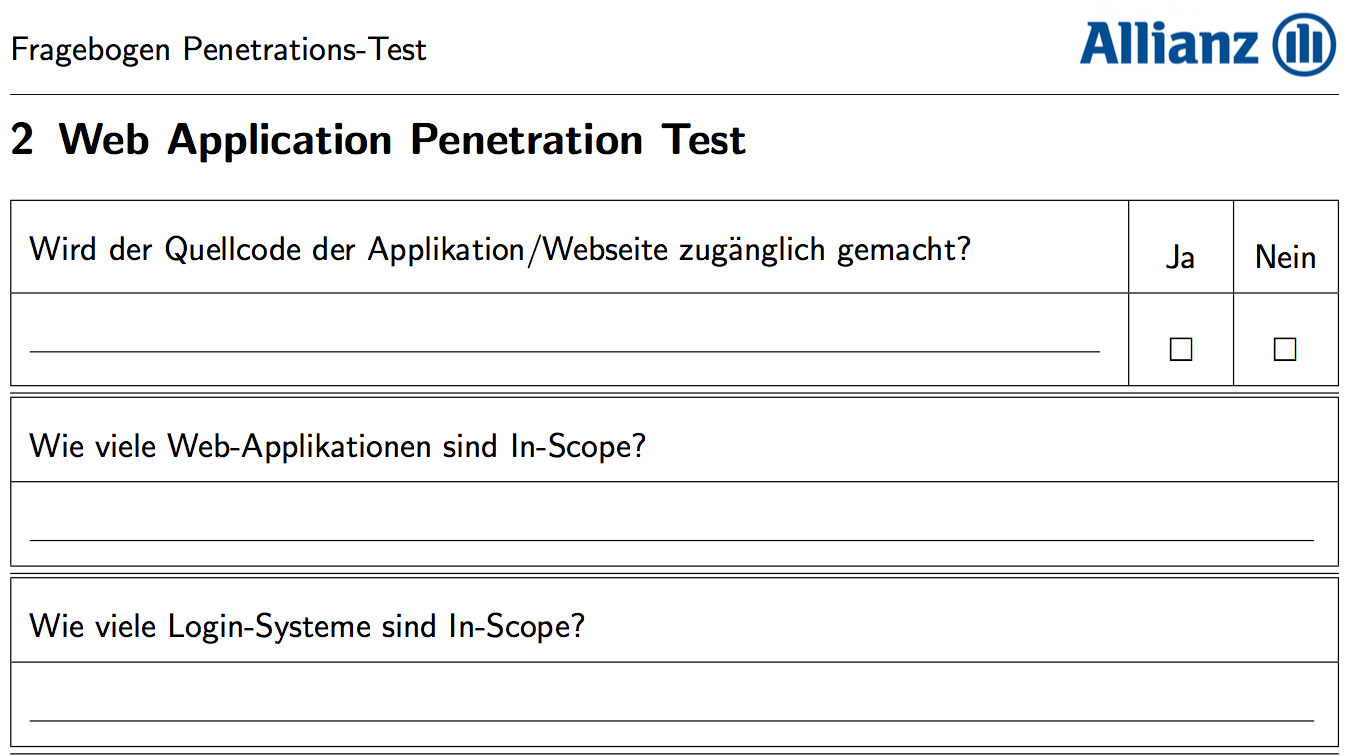
\includegraphics[width=\textwidth]{bilder/pentest_prozesse/vorbereitung/fragebogen_latex.png}
	\caption{Ein kurzer Ausschnitt des Fragebogens mit formatierten Fragen}
	\label{fig:FragLatex}
\end{figure}

Um eine möglichst einfache Erweiterung der Fragen in \textit{LaTeX} zu gewährleisten, wurden \textit{LaTeX}-Makros für die jeweiligen Frage-Arten entworfen. In Abbildung \ref{lst:PenProzVorbAutFormat} ist ein kurzes Beispiel für ein solches Makro dargestellt sowie zwei Fragen, die dieses nutzen.

\begin{figure}
\lstset{language=Tex}
\begin{lstlisting}
\newcommand{\frageJaNein}[1]{\makebox[\textwidth]{%
\renewcommand{\arraystretch}{2.0}
\begin{tabularx}{\textwidth}{|X|S|S|}
  \hline
  #1 & Ja & Nein\\
  \hline
  \line(1,0){350} & $\square$ & $\square$ \\
  \hline \hline
\end{tabularx}%
\renewcommand{\arraystretch}{1.0}
}}

\frageJaNein{Soll der Penetrations-Test aus verschiedenen Rollen durchgeführt werden?}
\frageJaNein{Sollen Angriffe auf gefundene Passwort-Hashes durchgeführt werden?}
\end{lstlisting}
\caption{Makro zur automatischen Formatierung in LaTeX}
\label{lst:PenProzVorbAutFormat}
\end{figure}

\subsubsection{Implementierung als Webabwendung}\label{ref:AufImplInWeb}
Die \textit{LaTeX}-Implementierung ist gut geeignet, um den Fragebogen vor Ort zu besprechen. Für ein Ausfüllen am Computer ist sie jedoch weniger geeignet, da man mit einem  PDF-Reader die Antworten einfügen müsste. Daher wurde eine Web-Anwendung entworfen, welche das Ausfüllen am Computer, zum Beispiel parallel zu einem Online-Meeting, vereinfacht.\\

Um die Anwendung möglichst minimalistisch und einfach zu halten, wurde \textit{Python} als Programmiersprache und \textit{Flask}\footnote{http://flask.pocoo.org/} als Web-Server verwendet. Auf HTML-Seite wurde \textit{Bootstrap 4}\footnote{https://v4-alpha.getbootstrap.com/} zur einfachen Formatierung genutzt.\\

Das Einfügen der Eingaben in der Weboberfläche wurde anfangs über eine einfache String-Substitution gelöst. Diese ist Abbildung \ref{lst:PenProzVorbereitStringSub} zu entnehmen.
\begin{figure}
\lstset{language=Python}
\begin{lstlisting}
# Load template from file
orig_file = open(tex_path + "/Fragen.tex", 'r')
template = LaTeXTemplate(orig_file.read())
orig_file.close()

# Substitute with form-fields
new_string = template.substitute(
    allg_anspr_web_app=__html_to_tex(
        request.form['allg_anspr_web_app']
    ),
    allg_pen_art_wapt=__html_to_checkbox(
        request, 'allg_pen_art_wapt'
    ),
    # Andere Form-Felder
)
\end{lstlisting}
\caption{String-Substitution zum Ersetzten von Inhalten für das TeX-Dokument}
\label{lst:PenProzVorbereitStringSub}
\end{figure}
Da dies jedoch einen erhöhten Wartungsaufwand bei zum Beispiel Änderung von Parametern mit sich zieht, wurde die Substitution durch eine einfachere Implementierung in \textit{Jinja2}\footnote{http://jinja.pocoo.org/docs/2.9/} ersetzt. Die Substitutions-Technik von \textit{Jinja} ist unter \ref{jinja2} aufgezeigt. Unter der Nutzung von \textit{Jinja}-Makros können so sehr effizient die HTML-Dateien für die Fragen erstellt werden. Unter \ref{lis:PenProzAufwFragHTMLJinja} ist ein kurzes Beispiel aus dem Fragebogen bezüglich Web-Application Penetration Tests aufgezeigt, in welchem einige Fragen definiert werden.

\begin{figure}[htbp]
\begin{lstlisting}
{{ binary_question("wapt_quell_zug", "Wird der Quellcode der Applikation/Webseite zugänglich gemacht?") }}
  {{ text_question("wapt_anz_web_app", "Wie viele Web-Applikationen sind In-Scope?") }}
  {{ text_question("wapt_anz_login_sys", "Wie viele Login-Systeme sind In-Scope?") }}
\end{lstlisting}
\caption{Definition von drei Fragen in HTML über Jinja2}
\label{lis:PenProzAufwFragHTMLJinja}
\end{figure}

Durch die Verwendung von \textit{Bootstrap} ist die Anwendung automatisch "`responsive"', also unter verschiedenen Auflösungen verwendbar. Ein Screenshot der Anwendung ist unter \ref{fig:FragWeb} dargestellt.\\

\begin{figure}[htbp]
	\centering
	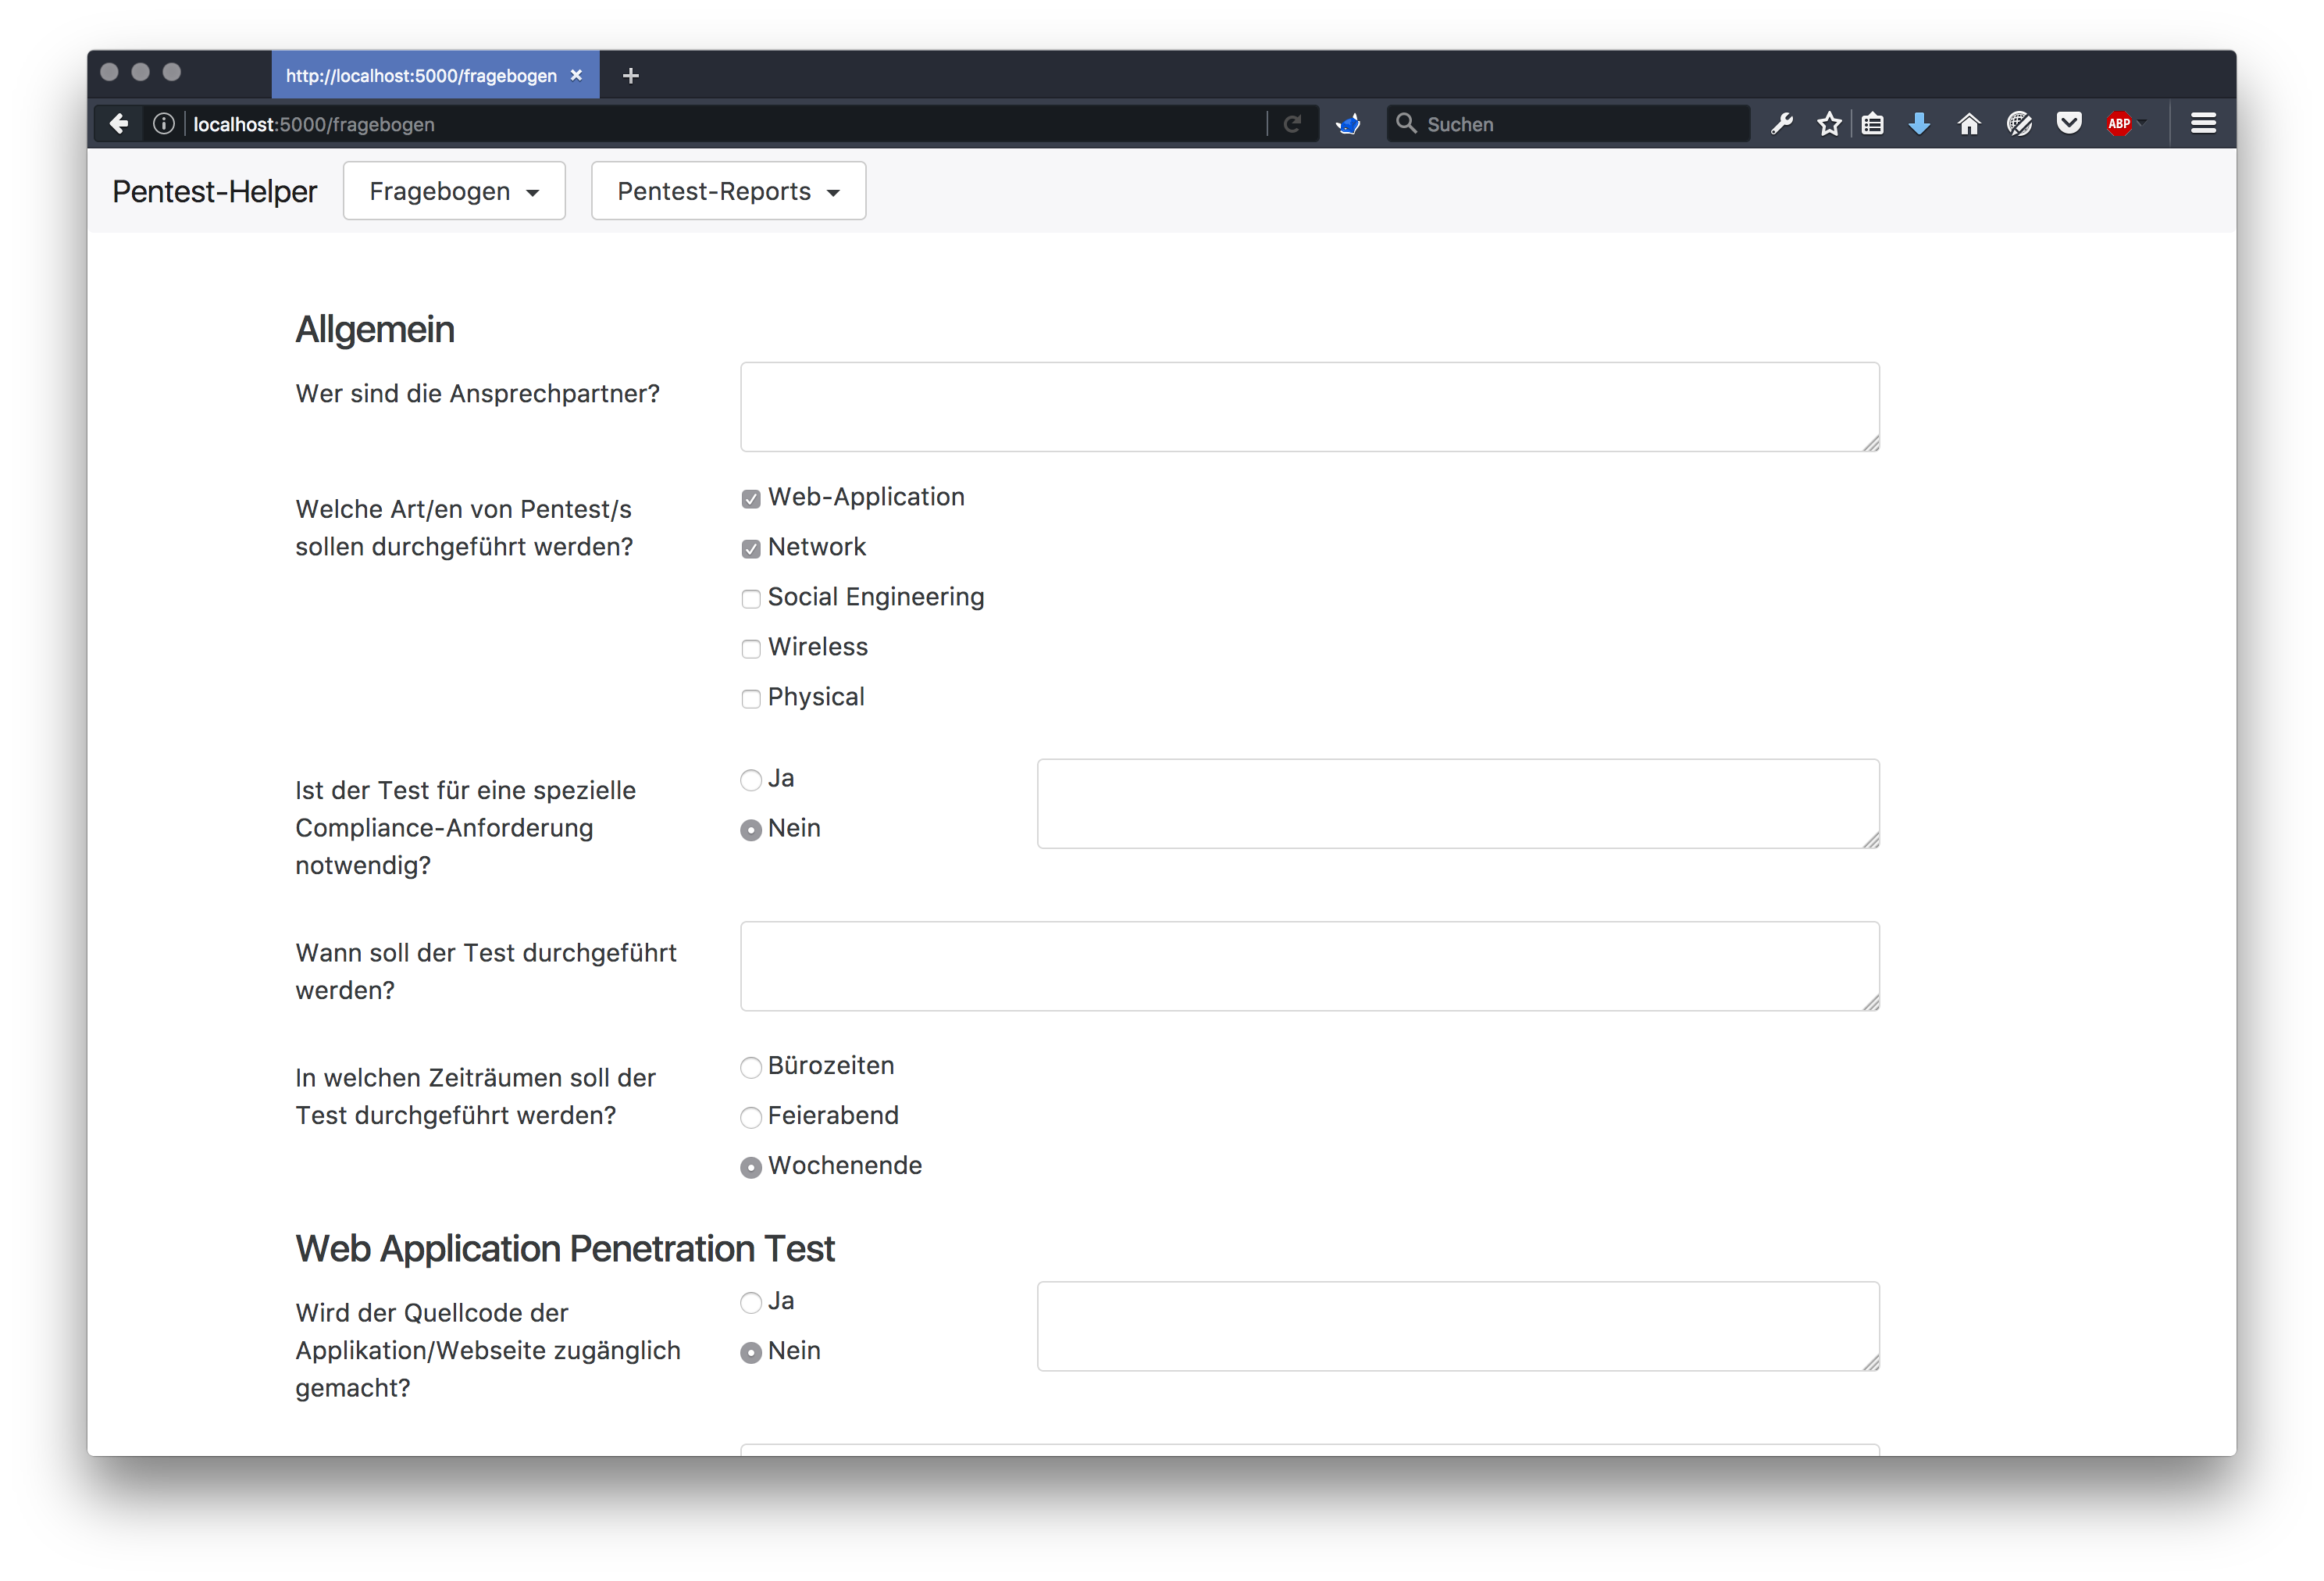
\includegraphics[width=\textwidth]{bilder/pentest_prozesse/vorbereitung/fragebogen_web.png}
	\caption{Ein kurzer Ausschnitt der Fragebogen-Webanwendung}
	\label{fig:FragWeb}
\end{figure}

Um die Daten dauerhaft zu speichern, wurde eine Datenbankanbindung implementiert. Hierzu wurde \textit{SQLAlchemy}\footnote{https://www.sqlalchemy.org/} als Engine genutzt, da diese sehr gut zu \textit{Flask} passt und sich einfach und ohne viel Aufwand implementieren lässt. Mehr zu \textit{SQLAlchemy} ist dem Abschnitt \ref{ref:SQLAlchemy} zu entnehmen.\\

Zum Erstellen des PDFs muss das generierte TeX-Dokument über \textit{pdflatex} umgewandelt werden. Der dazu genutzte Code ist in Listing \ref{lis:PenProzAufwPDFLatex} dargestellt.

\begin{figure}[htbp]
\begin{lstlisting}
try:
    subprocess.check_output(
        [
            '/usr/local/texlive/2016/bin/x86_64-darwin/pdflatex',
            '-synctex=1',
            '-interaction=nonstopmode',
            '--output-directory=' + output_path,
            tex_file_name
        ], cwd=tex_path
    )
except subprocess.CalledProcessError as error:
        print(error)
\end{lstlisting}
\caption{Aufruf von \textit{pdflatex} aus \textit{python} über das \textit{subprocess}-Modul}
\label{lis:PenProzAufwPDFLatex}
\end{figure}

Dabei wird der File-Path für das generierte TeX-File in der Variable \textit{tex\_path} übergeben und das generierte PDF unter \textit{output\_path} gespeichert.\\

Anschließend wird das PDF von \textit{Flask} über die \textit{send\_file}-Methode zurückgegeben und im Browser dargestellt. Das Ergebnis ist in Grafik \ref{fig:FragWebGen} dargestellt.

\begin{figure}[htbp]
	\centering
	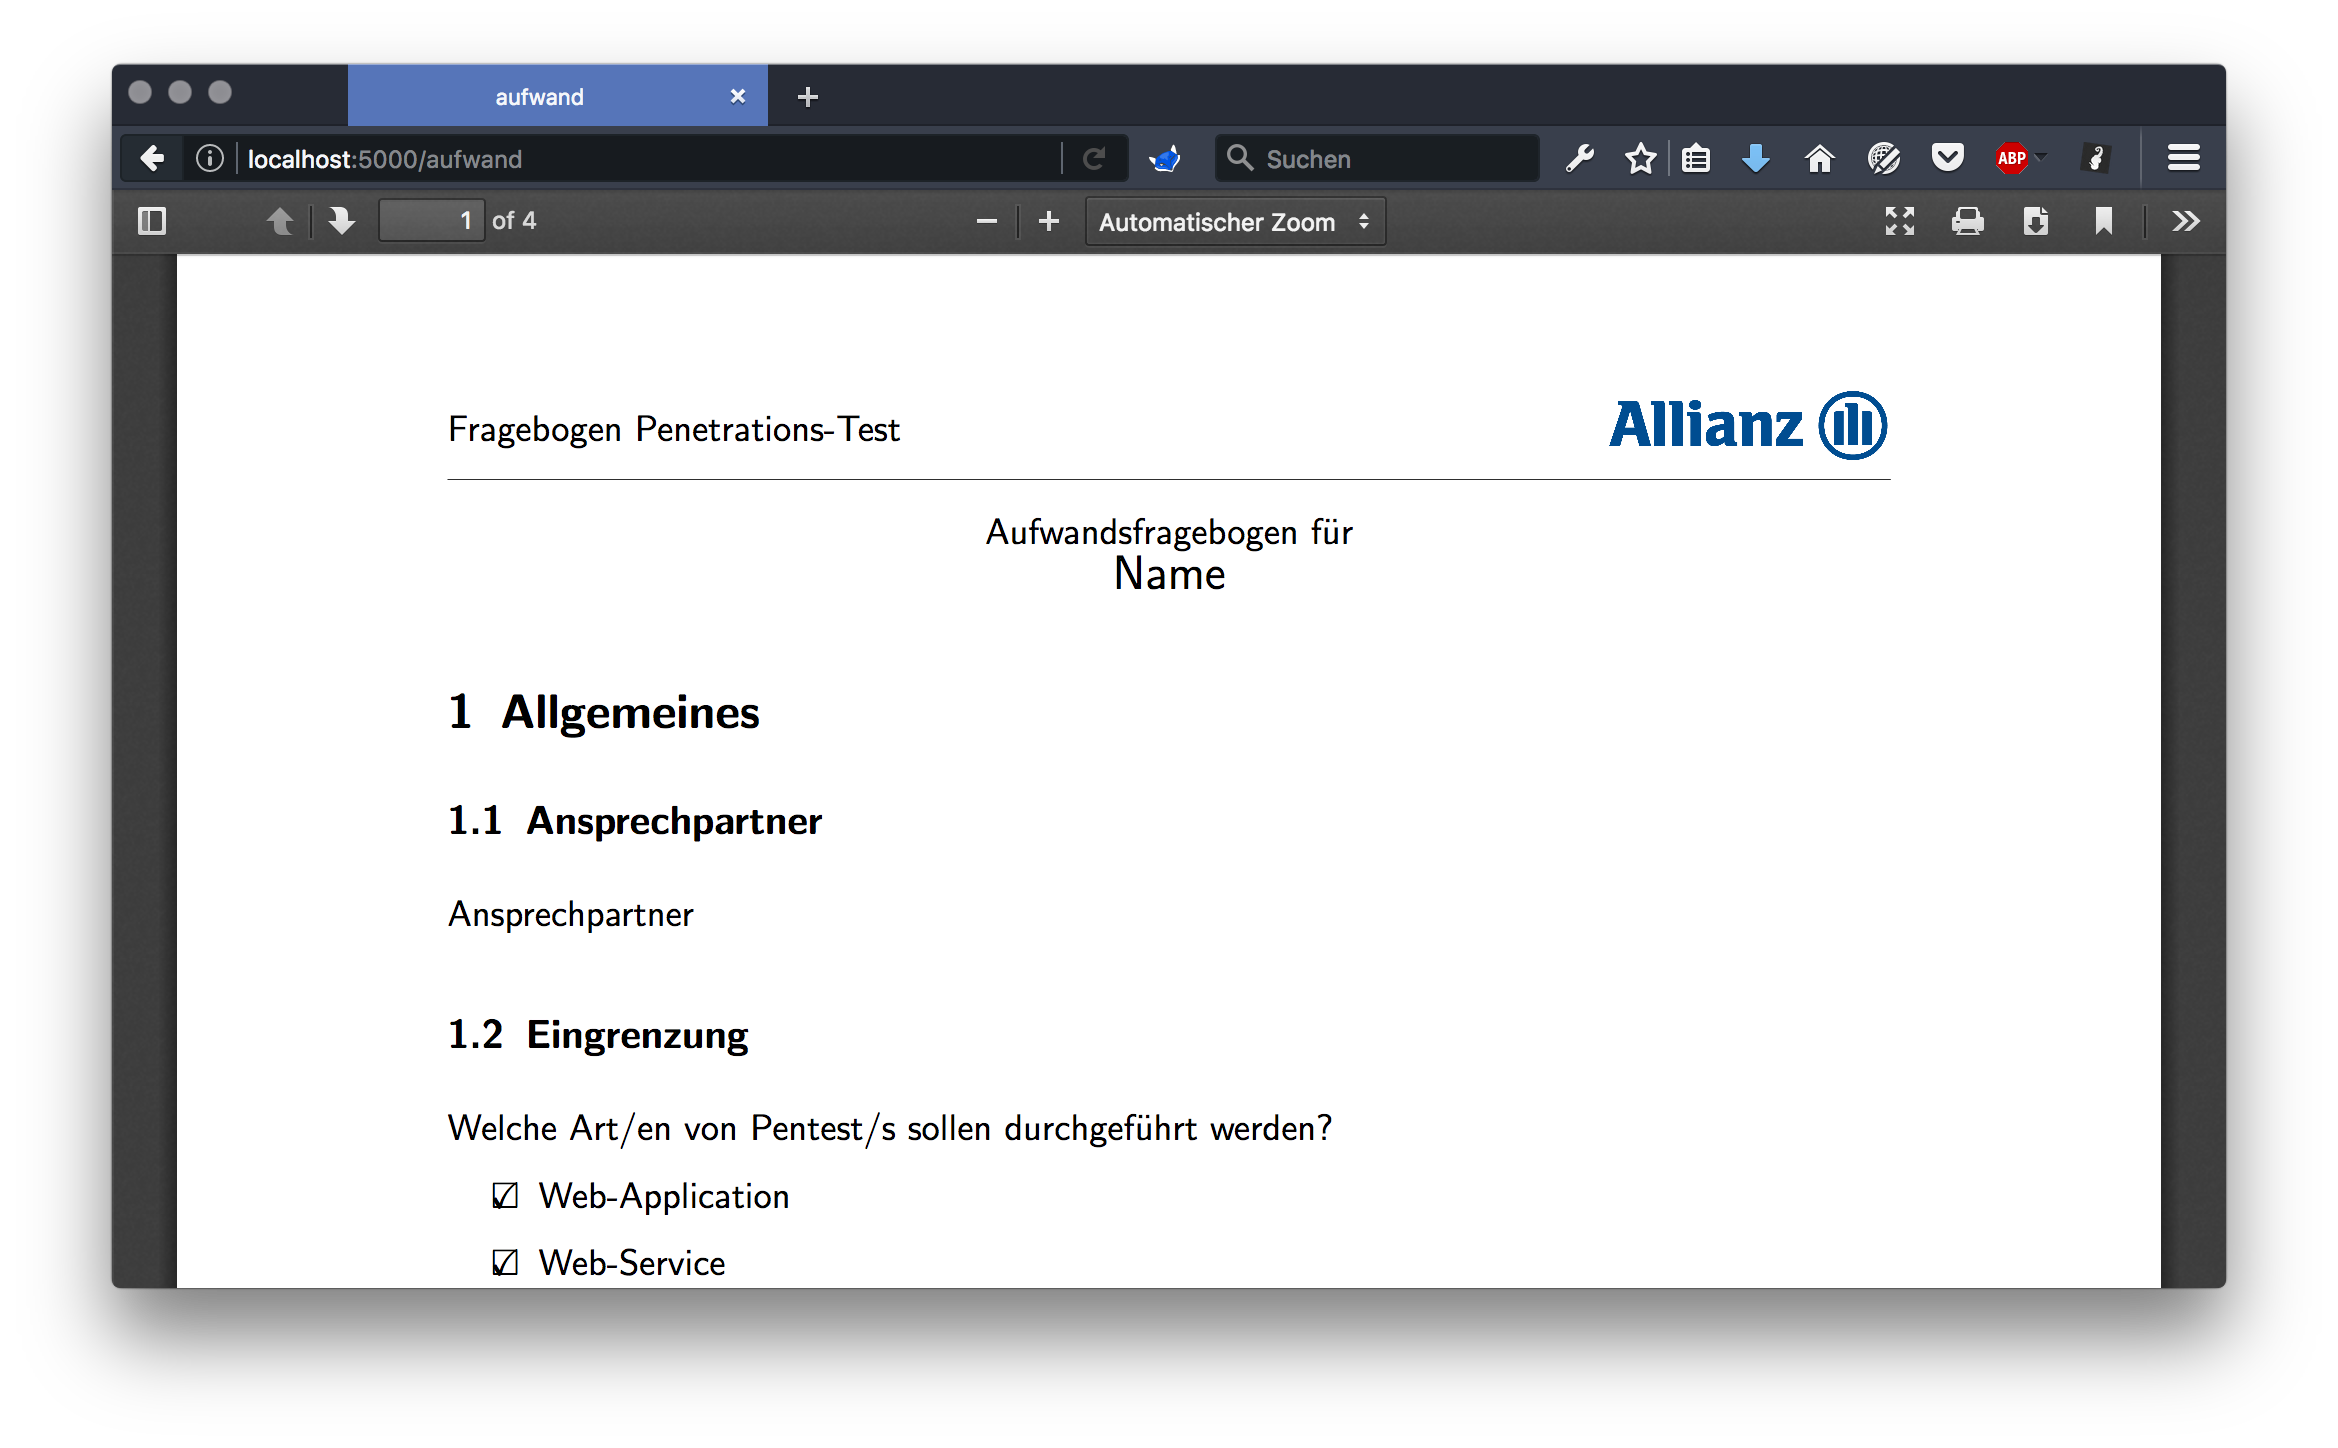
\includegraphics[width=\textwidth]{bilder/pentest_prozesse/vorbereitung/fragebogen_web_gen.png}
	\caption{Ausschnitt des Fragebogens nach Umwandlung über LaTeX zu PDF}
	\label{fig:FragWebGen}
\end{figure}

\newpage
\paragraph{Jinja2}\label{jinja2}
\textit{Jinja2}\footnote{\url{http://jinja.pocoo.org/docs/2.9/}} ist eine Template-Engine für \textit{Python}. Diese ist eigentlich für das Füllen von Inhalten in HTML-Dateien gedacht, kann sich jedoch auch auf andere Sprachen anwenden lassen.

Einige Features sind:
\begin{itemize}
    \item Ausführung in einer Sandbox
    \item Automatisches Escaping von HTML-Characters
    \item Template-Vererbung
    \item Code-Optimierung
    \item Sprechende Fehlermeldungen
    \item Anpassbare Syntax
\end{itemize}

Zudem erlaubt \textit{Jinja} eine Nutzung von übergebenen \textit{Python}-Objekten. So wird zum Beispiel im Fragebogen das unter Listing \ref{ref:jinja2-py} aufgezeigt Code-Segment genutzt.\\

\lstset{language=Python}
\begin{figure}[htbp]
\begin{lstlisting}
# Define template
template = latex_jinja_env.get_template('aufwand.tex')

# Render template
rendered_latex = template.render(
    aufwand=aufwand
)
\end{lstlisting}
\caption{Aufrufender Python-Code}
\label{ref:jinja2-py}
\end{figure}

\begin{figure}[htbp]
\lstset{language=Tex}
\begin{lstlisting}
\makebox[\textwidth]{%
\renewcommand{\arraystretch}{2.0}
\begin{tabularx}{\textwidth}{|X|}
  \hline
  Wie viele Einrichtungen sollen getestet werden? \\
  \hline
  \VAR{ aufwand.phys_anz_einr }	\\
  \hline \hline
\end{tabularx}%
\renewcommand{\arraystretch}{1.0}
}
\end{lstlisting}
\caption{Aufgerufenes Template}
\label{ref:aufwand.tex}
\end{figure}

\newpage
In Zeile 7 der Abbildung \ref{ref:aufwand.tex} ist der \textit{Jinja2}-Zugriff auf das Attribut \textit{$phys\_anz\_einr$} des in Zeile 6 der Abbildung \ref{ref:jinja2-py} übergebenen Objekts \textit{aufwand} zu sehen. Ebenso können Attribute geprüft und Makros implementiert werden. Beides ist im Code-Snippet \ref{ref:PenProzAufJinjaMacroCheck} dargestellt.\\

\begin{figure}
\begin{lstlisting}
\BLOCK{ macro checkbox(feld) }
    \BLOCK{ if feld == 'checked' }
        \mbox{\ooalign{$\checkmark$\cr\hidewidth$\square$\hidewidth\cr}}
    \BLOCK{ else }
        $\square$
    \BLOCK{ endif }
\BLOCK{ endmacro }
\end{lstlisting}
\caption{Jinja2-Macro zur Erstellung einer Frage mit Checkboxen}
\label{ref:PenProzAufJinjaMacroCheck}
\end{figure}

Dabei wird ein Makro implementiert, welcher ein übergebenes Attribut prüft (Zeile 2, \ref{ref:PenProzAufJinjaMacroCheck}) und je nach dem eine Checkbox mit einem Hacken (Zeile 3, \ref{ref:PenProzAufJinjaMacroCheck}) oder eine leere Checkbox (Zeile 5, \ref{ref:PenProzAufJinjaMacroCheck}) darstellt.

\paragraph{SQLAlchemy}\label{ref:SQLAlchemy}
\textit{SQLAlchemy} ist ein Modul zum Ausführen von SQL-Statements aus \textit{Python}. Eine Besonderheit ist der \textit{ORM} (\textit{Object Relational Mapper}), welcher es erlaubt, die Datenbank in Python als normale Klassen zu definieren. Die Definition des DB-Schemas sowie die Zugriffe auf die Datenbank passieren zum Großteil transparent.\\

So konnte zum Beispiel der Fragebogen zur Aufwandsschätzung aus \ref{ref:AufImplInWeb} direkt als Klasse definiert und im weiteren Kontext sowohl in \textit{Python} als auch in \textit{Jinja} verwendet werden. Das Beispiel in Listing \ref{lis:PenProzSQLAlchemy} verdeutlicht das Zusammenspiel zwischen \textit{Flask} und \textit{SQLAlchemy}.

\begin{figure}
\lstset{language=Python}
\begin{lstlisting}
from flask_sqlalchemy import SQLAlchemy
from flask import Flask, request
from jinja2 import Template

APP = Flask(__name__)
APP.config['UPLOAD_FOLDER'] = UPLOAD_FOLDER
APP.config['SQLALCHEMY_DATABASE_URI'] = 'sqlite:///test.db'
db = SQLAlchemy(APP)

class Aufwand(db.Model):
    id = db.Column(db.Integer, primary_key=True)
    allg_name = db.Column(db.Text)
    allg_anspr_web_app = db.Column(db.Text)
    allg_pen_art_wapt = db.Column(db.Text)
    [...]

    def __init__(self, aufwand):
        self.allg_name = aufwand.allg_name
        self.allg_anspr_web_app = aufwand.allg_anspr_web_app
        self.allg_pen_art_wapt = aufwand.allg_pen_art_wapt
        [...]
        
@APP.route('/aufwand', methods=['POST'])
def save_aufwand():

    aufwand_tuple = AufwandTuple(
        allg_name=request.form['allg_name'],
        allg_anspr_web_app=request.form['allg_anspr_web_app'],
        allg_pen_art_wapt='checked' if 'allg_pen_art_wapt' in request.form else '',
        allg_pen_art_wspt='checked' if 'allg_pen_art_wspt' in request.form else '',
        [...]
    )

    aufwand = Aufwand(aufwand_tuple)
    db.session.add(aufwand)
    db.session.commit()

    file_path = __generate_tex_aufwand(aufwand)
    return send_file(file_path, 'aufwand.pdf')
\end{lstlisting}
\caption{Minimales Beispiel für \textit{SQLAlchemy}}
\label{lis:PenProzSQLAlchemy}
\end{figure}

In den Zeilen 10 bis 21 wird die DB-Tabelle definiert, welche im weiteren Verlauf wie ein normales \textit{Python}-Objekt benutzt werden kann. In Zeile 34 wird ein DB-Eintrag erstellt und in den Zeilen 35 und 36 der Session hinzugefügt und in die Datenbank geschrieben. In Zeile 38 wird das Template aufgerufen, das Objekt übergeben und ein Template durch \textit{Jinja} gefüllt. Dies ist den Code-Snippets unter \ref{jinja2} zu entnehmen.

\subsubsection{Portierung nach Docker}\label{ref:PenProzPortDocker}
Um die Anwendung möglichst einfach auf weitere Rechner portieren zu können, wurde die Möglichkeit getestet, die Applikation, zusammen mit der Anwendung zur Erstellung von Pen-Test-Reports (siehe \ref{ref:PenProzReportWeb}) und dem Kickoff-Fragebogen (siehe \ref{ref:PenProzKickoffWeb}), in einen \textit{Docker}-Container aufzunehmen. Dazu wurde ein entsprechendes "`Dockerfile"' erstellt, welches im Anhang unter \ref{ap:Docker} zu finden ist.\\

Dabei wird \textit{Ubuntu 16.10} als Basis verwendet und anschließend alle Voraussetzungen installiert sowie der Service gestartet. Daraus ergeben sich für Benutzer zwei Möglichkeiten zur einfacheren Einrichtung des Programms. Entweder es kann lokal über das Kommando
\begin{lstlisting}
docker build -t dominikschlecht/pentest_helper .
\end{lstlisting}
erstellt werden oder es kann ein Abbild des Containers auf den Rechner kopiert und ausgeführt werden.\\

Leider stellte sich heraus, dass die \textit{LaTeX}-Installation sowie andere Komponenten den Container auf eine Größe ansteigen lassen, welche den Austausch schwierig gestalten würden. Daher wurde vorerst auf eine Portierung auf \textit{Docker} verzichtet.

	\subsection{Rechtliche Aspekte}
	Sollte eine Beauftragung erfolgen, müssen sowohl Auftragnehmer wie Auftraggeber verschiedene rechtliche Aspekte beachten. Im Folgenden sind kurz einige der wichtigsten Aspekte dargestellt, welche zusätzlich zum normalen Vertrag beachtet werden sollten.\\
	
\begin{description}
	\item[NDA: ] Im Normalfall wird der Auftraggeber ein NDA (Non-Disclosure-Agreement, zu deutsch Vertraulichkeitserklärung) vom Auftragnehmer einfordern. Dieses verpflichtet Auftragnehmer dazu, keine Informationen über den Pen-Test an Dritte weiterzugeben. Dieses Vertragsstück schützt den Auftraggeber vor Reputationsschäden und sollte auf jeden Fall geschlossen werden. Beachtet werden sollte jedoch, dass die Vertragsstrafe bei Verletzung der Abmachung auch dem wirklich zu erwartenden Schaden entspricht.
	
	\item[Haftungsausschluss: ] Im Gegenzug wird der Auftragnehmer einen Haftungsausschluss vom Auftraggeber einfordern. In diesem ist definiert, dass der Auftragnehmer nicht für entstehende Schäden aufkommt. Dies ist für Pen-Tester äußerst wichtig, da bei Tests oft beiläufig und unabsichtlich Randsysteme in Mitleidenschaft gezogen werden. Ein Beispiel wäre eine Log-Instanz, welche die Log-Meldungen des anzugreifenden Systems verarbeitet, aber unter der Last der Log-Meldungen aufgrund von Security-Scans abstürzt. Wurde kein Haftungsausschluss vereinbart, wäre der Auftraggeber unter Umständen imstande, den Auftragnehmer auf den entstandenen Schaden zu verklagen. 
	
	\item[Personenbezogene Daten: ] Falls im Laufe des Pen-Tests der Auftragnehmer Zugriff auf personenbezogene Daten erlangen könnte, sollte dies mit dem Datenschutzbeauftragten des Auftraggebers besprochen und, falls notwendig, entsprechende Vereinbarungen getroffen werden.
\end{description}

	\newpage
	\subsection{Technische Aspekte}
	Im Vorfeld zu einem Pen-Test sollten auch verschiedene technische Aspekte beachtet werden. Diese sind im folgenden in Ausstattung, Infrastruktur und Tools aufgeteilt.
	
		\subsubsection{Ausstattung}
		Natürlich benötigt ein Pen-Tester eine gewisse Ausrüstung. Dazu sollten auf jeden Fall Rechner mit mittlerer bis hoher Prozessorleistung sowie ausreichend RAM für das Ausführen von virtuellen Maschinen gehören. Zudem wäre eine Grafikkarte zu erwägen, um, falls gewünscht, Attacken auf Passwort-Hashes durchführen zu können, welche auf der GPU wesentlich effizienter sind als auf der CPU. Insofern der Auftraggeber jedoch damit einverstanden ist, kann dies ebenfalls z.B. in einer Cloud-Umgebung durchgeführt werden, da hier innerhalb weniger Minuten Rechner mit einer Vielzahl an GPUs zur Verfügung stehen. Der Nachteil ist natürlich, dass die Hashes dadurch in das Rechenzentrum des Cloud-Betreibers geladen werden müssen.\\
		
		Sollte ein Vor-Ort-Einsatz geplant sein, könnte ebenso ein Ethernet-Tap \footnote{\url{https://greatscottgadgets.com/throwingstar/}}, entsprechend viele LAN-Kabel sowie ein WLAN-Router von Vorteil sein.\\
		
		Sollen Pen-Tests auf mobile Applikationen durchgeführt werden, sollte für \textit{iOS}-Apps ein \textit{Mac Book} zur Verfügung stehen. Zwar können alle mobilen Betriebssysteme emuliert werden, dies ist jedoch zum Teil mit Nachteilen verbunden (siehe Abschnitt \ref{ref:VerglAktSitEmu}). Daher empfiehlt sich ein physikalisches Endgerät für jeweils \textit{iOS}, \textit{Android} und \textit{Windows-Phone}. Diese sollten jeweils mit einem \textit{Jailbreak} ausgestattet sein, um alle Analysen vornehmen zu können.\\
		
		Bei einem Team von Pen-Testern sollte auf Kompatibilität bezüglich der verwendeten Hardware und Komponenten geachtet werden. Zusätzlich können Plattformen wie das \textit{Integrated Pentest Environment}\footnote{https://www.faradaysec.com/} von \textit{Faraday} die Zusammenarbeit im Team vereinfachen.

		\subsubsection{Infrastruktur}\label{ref:vorbInfrastruktur}
		Gerade beim Pen-Testen von Web-Applikationen sollte der Pen-Tester eine statische IP besitzen, von welcher aus er testet. Sollte die Umgebung, von welcher getestet wird, diese Eigenschaft nicht aufweisen, sollte ein Proxy-Server verwendet und alle jeglicher Netzwerkverkehr über diesen geleitet werden. Nur so kann der Auftraggeber feststellen, ob die Angriffe wirklich von Auftragnehmer kommen oder parallel ein echter Angriff stattfindet.\\
		
		Ebenso sollte eine gemeinsame Ablage erstellt werden, über welche Pen-Tester alle notwendigen Informationen austauschen können. Dabei sollte die Ablage so dynamisch wie möglich sein. Eine Möglichkeit wäre \textit{etherpad} \footnote{\url{https://etherpad.org/}}, da es als Open-Source-Software keine weiteren Lizenzen erfordert und einen schnellen, dynamischen Austausch ermöglicht. Zudem können die Daten einfach als \textit{HTML}-File exportiert werden.
		
		\subsubsection{Betriebssystem und Tools}
		Bei Pen-Tests ist es essentiell, dass die Pen-Tester ihr Laptop sehr genau kennen und keine unerwarteten Aktionen auftreten. Ein Beispiel wäre \textit{DHCP}, welches in Endbenutzer-Distributionen wie \textit{Ubuntu} standardmäßig aktiviert ist und direkt beim Einstecken des Netzwerkkabels versucht, eine IP zu beziehen. Bei einem Network-Penetration-Test kann es aber durchaus von Nutzen sein, wenn der Rechner keine sofortig Kommunikation mit dem Netzwerk aufbaut. Daher sollte ein möglichst minimales System gewählt und nur notwendige Software installiert werden. Dazu bieten sich als Betriebssysteme hoch konfigurierbare Linux-Distributionen wie \textit{Gentoo}\footnote{\url{https://www.gentoo.de/}} oder \textit{Arch-Linux}\footnote{\url{https://www.archlinux.de/}} an.\\
		 
		Bei der Installation von Software sollte immer auf vertrauenswürdige Quellen geachtet werden. Im besten Fall lädt man den Source-Code aus dem offiziellen Code-Verwaltungssystem und kompiliert diesen lokal. Bei einer vollkommen identischen Hardware und Konfiguration des Betriebssystems ergibt sich hier der Vorteil, dass die kompilierte ausführbare Datei zwischen den Pen-Testern ausgetauscht werden kann. Ist der Quellcode nicht öffentlich, sollte die Software auf jeden Fall nur von der Herstellerseite heruntergeladen werden. Zusätzlich empfiehlt es sich immer, die Signatur oder Checksumme der heruntergeladene Software zu prüfen, um Manipulationen auszuschließen.\\
		
		Ein weiterer wichtiger Punkt ist die Aktualität der Software. Hier gibt es zwei Aspekte, welche sich manchmal gegenüber stehen. Zum einen sollte gerade Software, welche zum Aufdecken von Schwachstellen genutzt wird, immer aktuell sein, um auch neueste Angriffe abprüfen zu können. Auf der anderen Seite steht die hohe Anforderung an Verfügbarkeit der Programme im Test und die Vergleichbarkeit zwischen verschiedenen Tests. So will man vermeiden, dass eine Software zum Start eines Pen-Tests wegen zum Beispiel Paketkonflikten nicht mehr funktioniert, oder dass zwei Pen-Tester mit unterschiedlichen Versionen arbeiten und daher unterschiedliche Ergebnisse für den gleichen Test erlangen. Eine Lösung für das Problem könnten virtuelle Maschinen darstellen. So kann man vor jedem Pen-Test einen Snapshot erstellen, ein Update durchführen und falls es Probleme gibt, welche sich bis zum nächsten Pen-Test nicht beheben lassen, auf diesen zurückspringen. Nach dem Pen-Test kann dann in Ruhe an dem jeweiligen Problem weitergearbeitet werden. Zudem hat dies den Vorteil, dass man die virtuelle Maschine nach dem Pen-Test löschen kann und so garantiert keine Fragmente des Pen-Test und damit des Kunden im Betriebssystem verbleiben.\\
		
		Unabhängig davon, ob die Daten des Pen-Tests nur in einer virtuellen Maschine oder auf dem physikalischen Client gehalten werden, sollte das Laptop an sich geschützt sein. Maßnahmen dazu sind die richtige Konfiguration des \textit{BIOS}, Festplattenverschlüsselung und das Deaktivieren von bestimmten Anschlüssen oder Hardware-Features. So sollte das \textit{BIOS} mit einem Kennwort geschützt und die Boot-Reihenfolge möglichst restriktiv gesetzt sein. Dies ist auch bei Laptops mit Festplattenverschlüsselung empfohlen, da sonst der Bootloader der Full-Disk-Encryption mit Malware (zum Beispiel über USB) infiziert werden könnte.\footnote{\url{https://www.schneier.com/blog/archives/2009/10/evil_maid_attac.html}}
